%KASCADE gamma search

% \begin{frame}{KASCADE-Grande}
% \begin{itemize}
%   \item Proposed in 1989---disassembled in 2013;
%   \item Aimed at studying
%   high-evergy (galactic) cosmic rays by observing extensive air showers (EAS);
% %   processes at the edge of the Galaxy and beyond by observing extended atmospheric showers (EAS);
%   \item Consisted of:
%   \begin{itemize}
%     \item scintillators detecting $e$, $\gamma$, $\mu$:
%     \begin{itemize}
%   %сцинтиляторы, различают e, gamma, mu
%     \item KASCADE---256 stations;
%     \item GRANDE---37 stations;
%     \end{itemize}
%  %один большой калориметр
%     \item Hadronic callorimeter;
%  %радиодетектор
%     \item Digital radio array LOPES detecting $e$, $e^{+}$;
% % позволяющих наблюдать различные компоненты ливня
%   \end{itemize}
%   \item Important features of cosmic-ray spectrum have been obtained. The data analysis is ongoing;
% %  благодаря данным с эксперимента было открыто много всего ополезного, при этом анлиз данных продолжается. новые статьи выходят
%   \item KCDC (\textbf{K}ASCADE \textbf{C}osmic Ray \textbf{D}ata \textbf{C}enter, \textcolor{blue}{\texttt{http://kcdc.ikp.kit.edu}}) is a dedicated portal where all the data collected are available online. % At the moment
% \end{itemize}
% 
% \begin{frame}{KASCADE-Grande gamma-ray limits}
% %   \item Limits on the ratio of diffuse gamma-ray flux to cosmic ray flux
%   \begin{minipage}{0.5\textwidth}
%    left
%   \end{minipage}
% 
% %   \begin{columns}
% %     \column{0.5\textwidth}
% %     left
% %     \column{0.5\textwidth}
% %     right
% %   \end{columns}
% \end{frame}


\section{KASCADE high-energy \texorpdfstring{$\gamma$}{gamma}-ray search}

\begin{frame}{High-energy $\gamma$-ray sources in KASCADE field of view}
%   KASCADE data: Efficiency of registration, exposure map *
  
  \begin{center}
    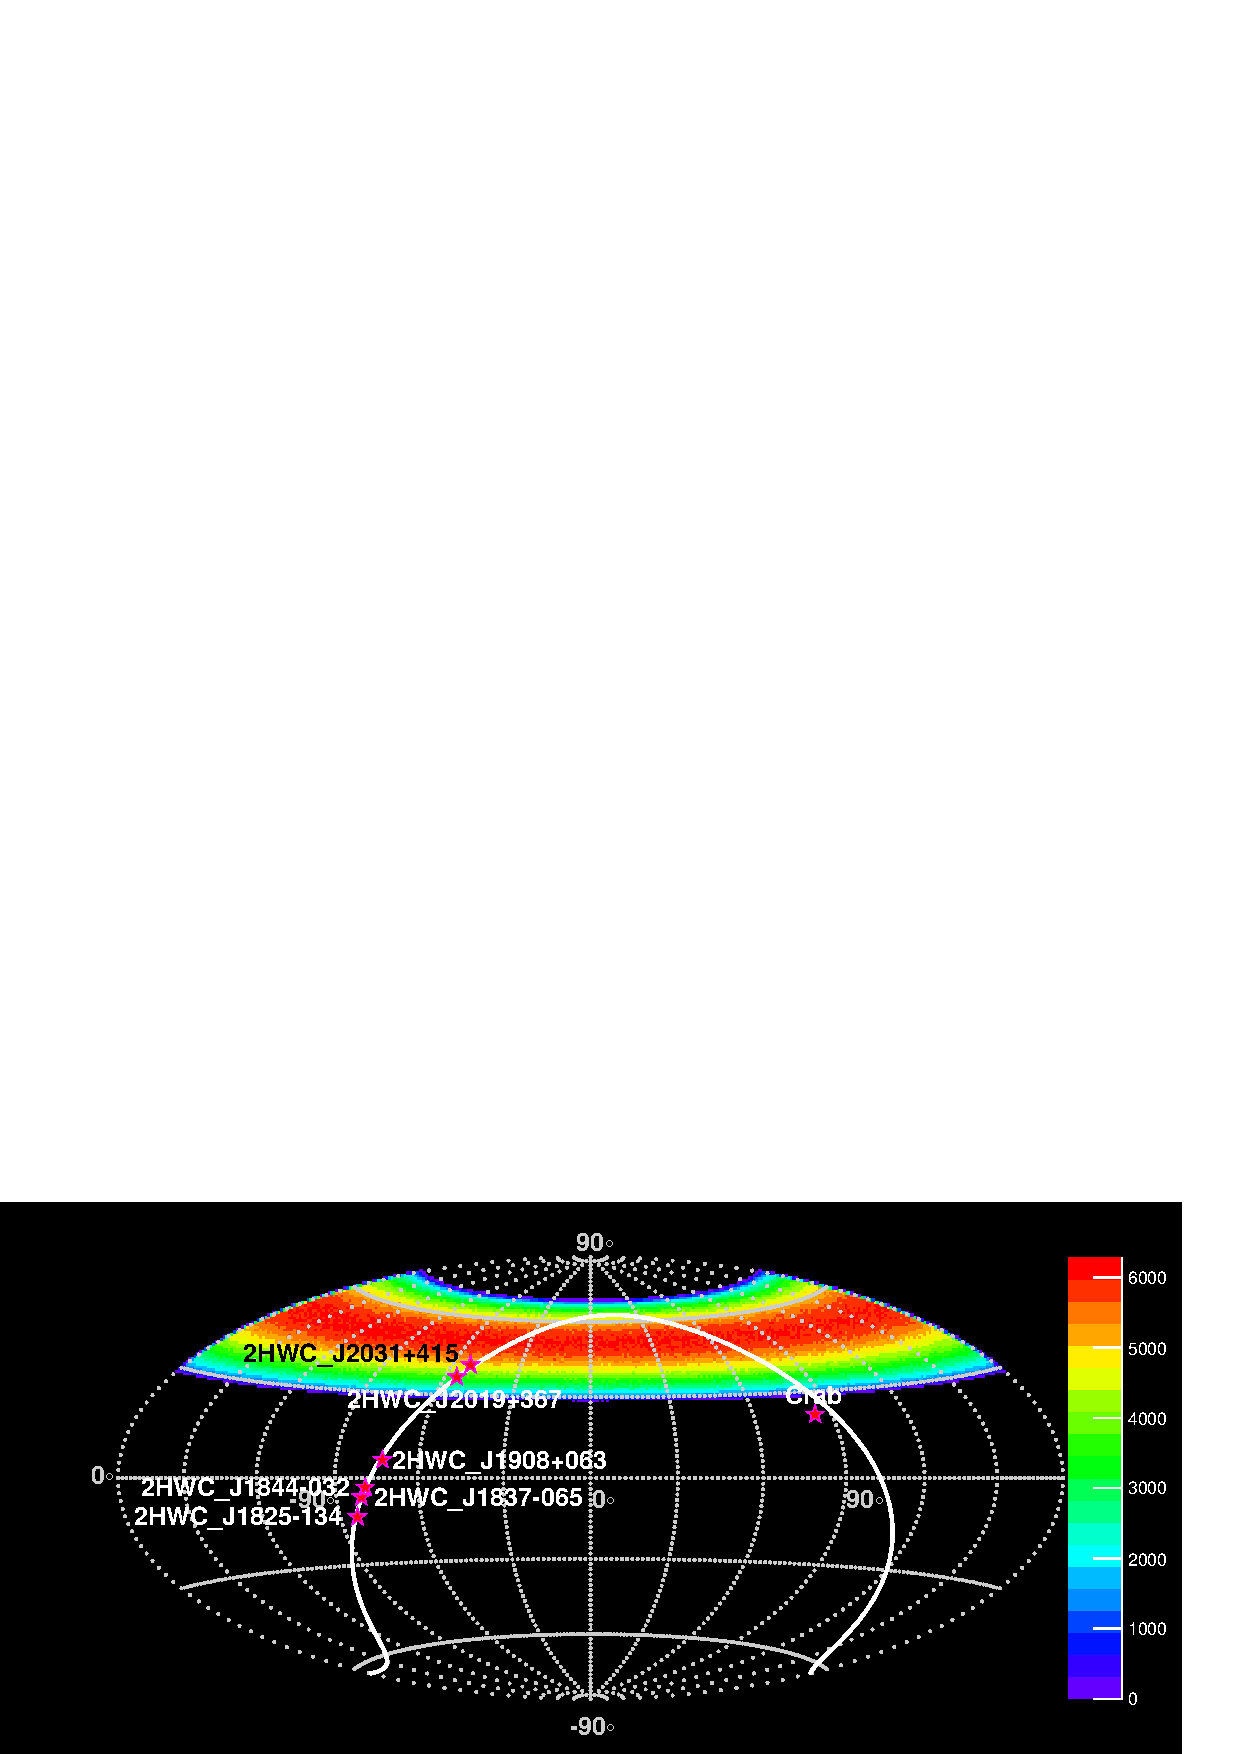
\includegraphics[width=1\textwidth]{pics/Skymap_6srcs.pdf}
    
 KASCADE events distribution map
  with\\ 6 HAWC sources with $E \approx 100$ TeV.
\end{center}
\end{frame}

\begin{frame}{KASCADE-Grande $\gamma$ ray searches}
\begin{itemize}
 \item Limits on the ratio of diffuse gamma-ray flux to cosmic ray flux
\end{itemize}

\begin{center}
    \includegraphics[width=0.65\textwidth]{pics/KASCADE-Grande_UHECR2016.pdf}
\end{center}
\end{frame}

\begin{frame}{KASCADE-Grande $\gamma$ ray searches}
\begin{itemize}
 \item - Limits on the diffuse gamma-ray flux: the best upper limit of the fraction of $\gamma$-rays
to the total cosmic ray flux is obtained at $3.7 \times 10^{15} eV$ with $1.1 \times 10^{-5}$. 
\end{itemize}

\begin{center}
    \includegraphics[width=0.55\textwidth]{pics/KASCADE-Grande_UHECR2016-2.pdf}
\end{center}
\end{frame}

\begin{frame}{$\gamma$-proton separation}
\small
% \begin{figure}[h]
\vspace{-1em}
\begin{center}
    \includegraphics[width=0.65\textwidth]{pics/Nmu_Ne.pdf}
    
    Distribution of $N_\mu / N_e$ for various primary CR components.
\end{center}
%   Распределение компонент ливня в зависимости от соотношения мюоной и электронной компоненты ливня
% \caption{
% \vspace{1em}
% }
%  \end{figure}
Taking into account this distribution and the flux upper-limit mentioned above we can make the 
$N_\mu/N_e \in [0, 0.008)$ cut to discriminate $\gamma$ component with ... C.L.
\end{frame}

\begin{frame}{HAWC high-energy sources in KASCADE field of view}
 \begin{center}
    \includegraphics[width=1\textwidth]{pics/2HWCsources.pdf}
    
 Events by KASСADE in $5^0$ radius around the point sources $2HWC_J2019+367$, $2HWC_J2031+415$ correspondingly.

\end{center}
\end{frame}


\begin{frame}{KASCADE statistics estimation for $2HWC_J2013+415$}

\begin{table}[]
\begin{tabular}{lll}
E &       N &      $F_{int}$  \\
7 & 440.9659202598506 & 1.406167411764706e-13\\
56 & 12.857367242057173 & 4.100001833751227e-15\\
100 & 4.798126510222744 & 1.5300432133675341e-15\\
1000 & 0.09573521008300581 & 3.052837563906128e-17\\
\end{tabular}
\end{table}

% There supposed to be 2 slides on this
%  Оценка количества событий вокруг 2HWC_J2013+415 +-
\end{frame}
